\section{旋转建模法}
\subsection{绘制杯零件左视图}\label{sec:beilingjianleft}
通过对图\ref{fig:tiaoyafabei}的分析,位于左边的主视图清晰的表过该杯零件为典型的简单回转体块零件,位于右边的左视图清楚地表达了杯块零件内部结构。为了建模该杯零件的三维模型,我们需要绘制左视图中具有剖面线部分的封闭图形,并以此图形做为三视建模的基础,注意到该图形为对称图形,因此只需要绘制一半的图形作为基础特征用以旋转建模。通常有两种方法完成图形的绘制。
\subsubsection{直接绘制法}
\begin{procedure}
\item 启动AutoCAD软件,常见的启动方法有:
\begin{itemize}
\item 双击桌面图标
\includegraphics[scale=0.2]{cadicon.png}。
\item 【开始】菜单【所有程序】子菜单中【Autodesk】子菜单中【AutoCAD 2013 – 简体中文 (Simplified Chinese)】子菜单中的【AutoCAD 2013 – 简体中文 (Simplified Chinese)】项。
\end{itemize}
AutoCAD启动后,其界面如图\ref{fig:cadui}所示。
\noindent
\begin{figure}[htbp]
\centering
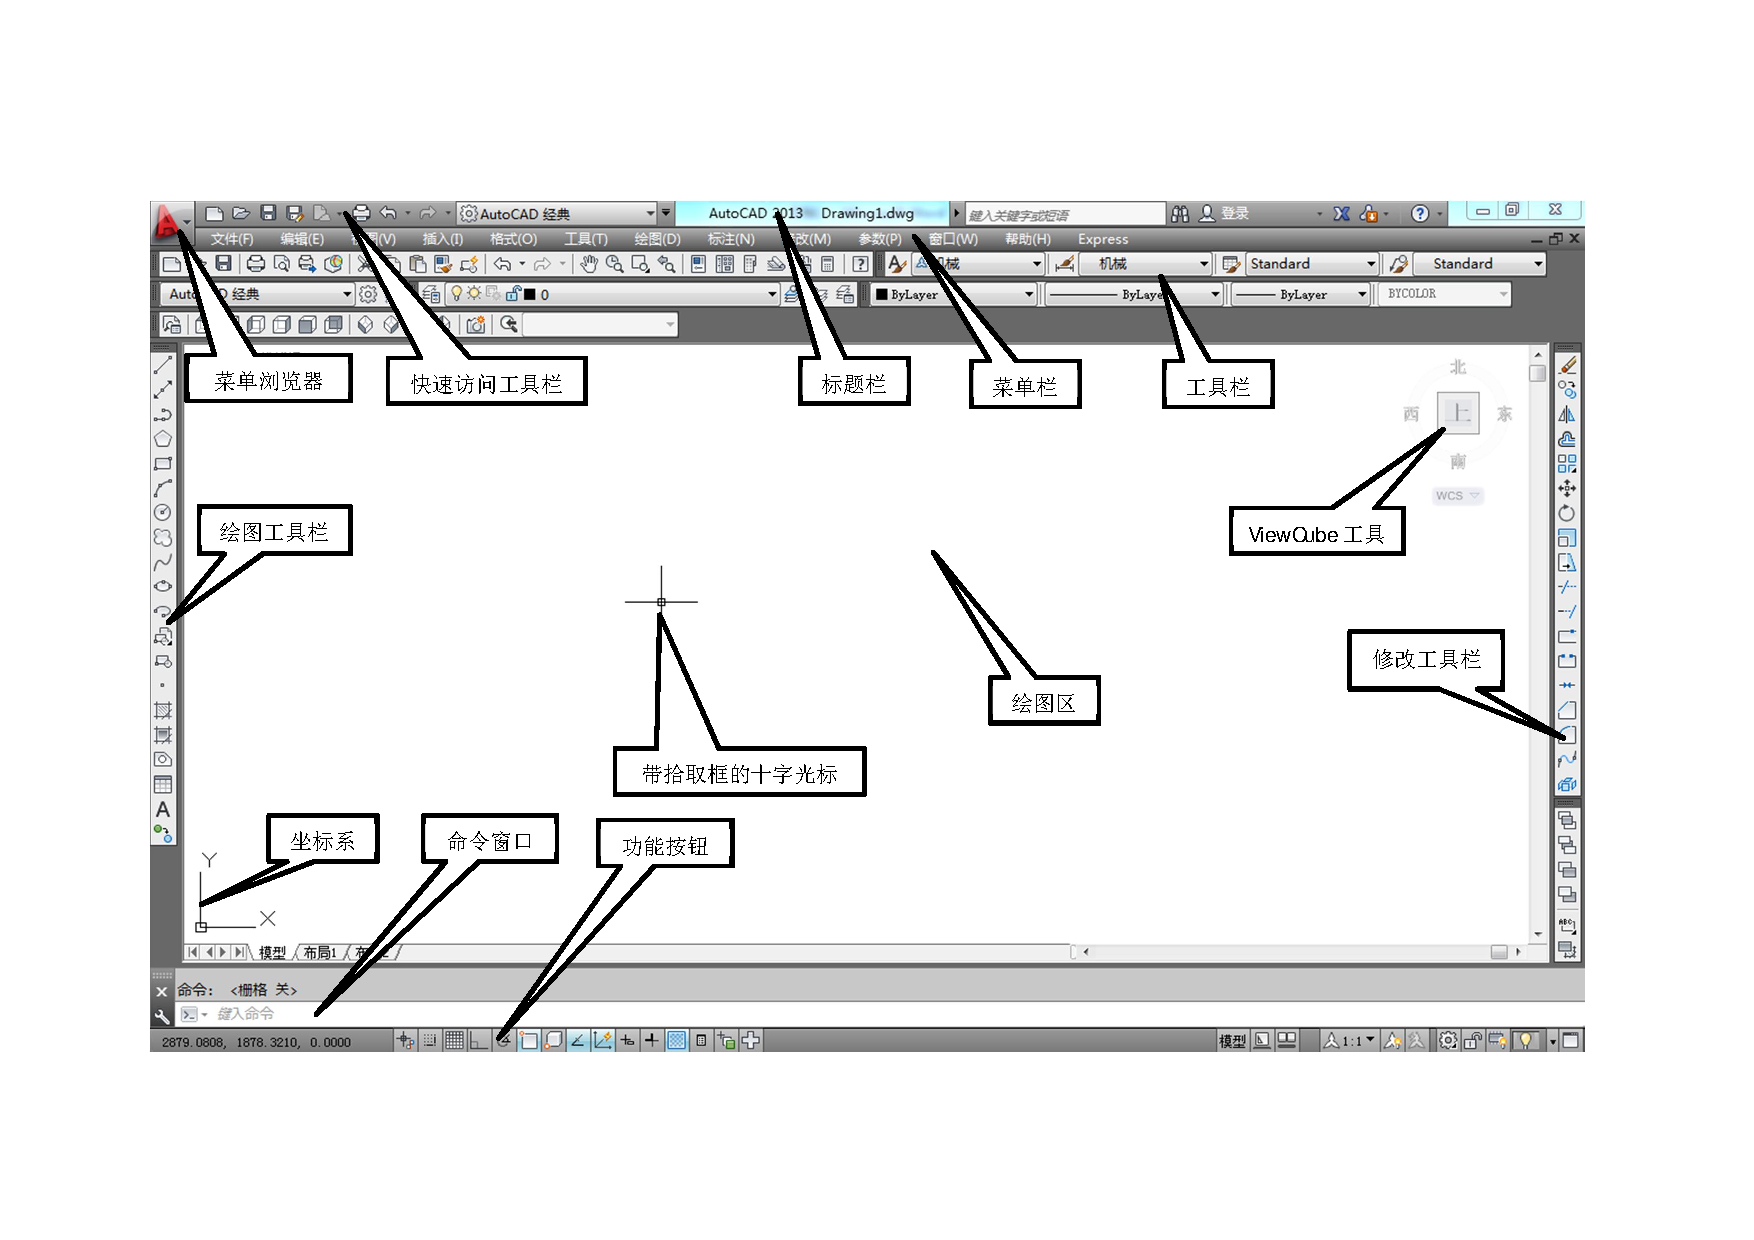
\includegraphics[scale=0.5]{cadui.pdf}
\caption{“AutoCAD经典”工作空间}\label{fig:cadui}
\end{figure}
\item 将视图切换为左视图。实现视图切换的方法有:
\begin{itemize}
\item 键盘输入-VIME或-V,选择【正交】选项中的【左视】项。
\item 在【视图】菜单【三维视图】子菜单中单击【左视图】项。
\item 在【视图】工具栏中单击【左视】图标
\includegraphics[scale=0.6]{toptool.png}。
\end{itemize}
\item 启动【直线】命令,具体方法有:
\begin{itemize}
\item 键盘输入line或L。
\item 在【绘图】菜单中单击【直线】项。
\item 在【绘图】工具栏中单击【直线】图标
\includegraphics[scale=0.6]{linetool.png}。
\end{itemize}
\item 输入图线坐标点,实现封闭图形的绘制。

\begin{lstlisting}
|命令: LINE|
|指定第一个点:0,0\longremark{数字,数字的形式为坐标点的绝对坐标表示法。}|
|指定下一点或 [放弃(U)]: @15,0\longremark{@数字,数字的形式为坐标点的相对坐标表示法,符号@用于表示相对,@号后面的数字分别为该点相对于前一点的$x$和$y$坐标增量。}|
|指定下一点或 [放弃(U)]: $@4<90$\longremark{@数字$<$数字的形式为相对极坐标表示法,符号@用于表示相对,$<$号前的数字用来表示线段的长度,$<$号后面的数字用来表示线段与$x$轴之间的夹角。}|
|指定下一点或 [闭合(C)/放弃(U)]: $@-10<0$|
|指定下一点或 [闭合(C)/放弃(U)]: $@11<90$|
|指定下一点或 [闭合(C)/放弃(U)]: $@-5<0$|
|指定下一点或 [闭合(C)/放弃(U)]: c\longremark{表示与第一个点进行闭合,当直线命令绘制完成三个点后该选才会出现。}|
\end{lstlisting}
\end{procedure}

通过以上步骤,我们已经完成了杯零件的主要特征绘制,其结果如图\ref{fig:bettezheng}所示。现对步骤中标注部分说明如下:
\showremarks
\noindent
\begin{figure}[htbp]
\centering
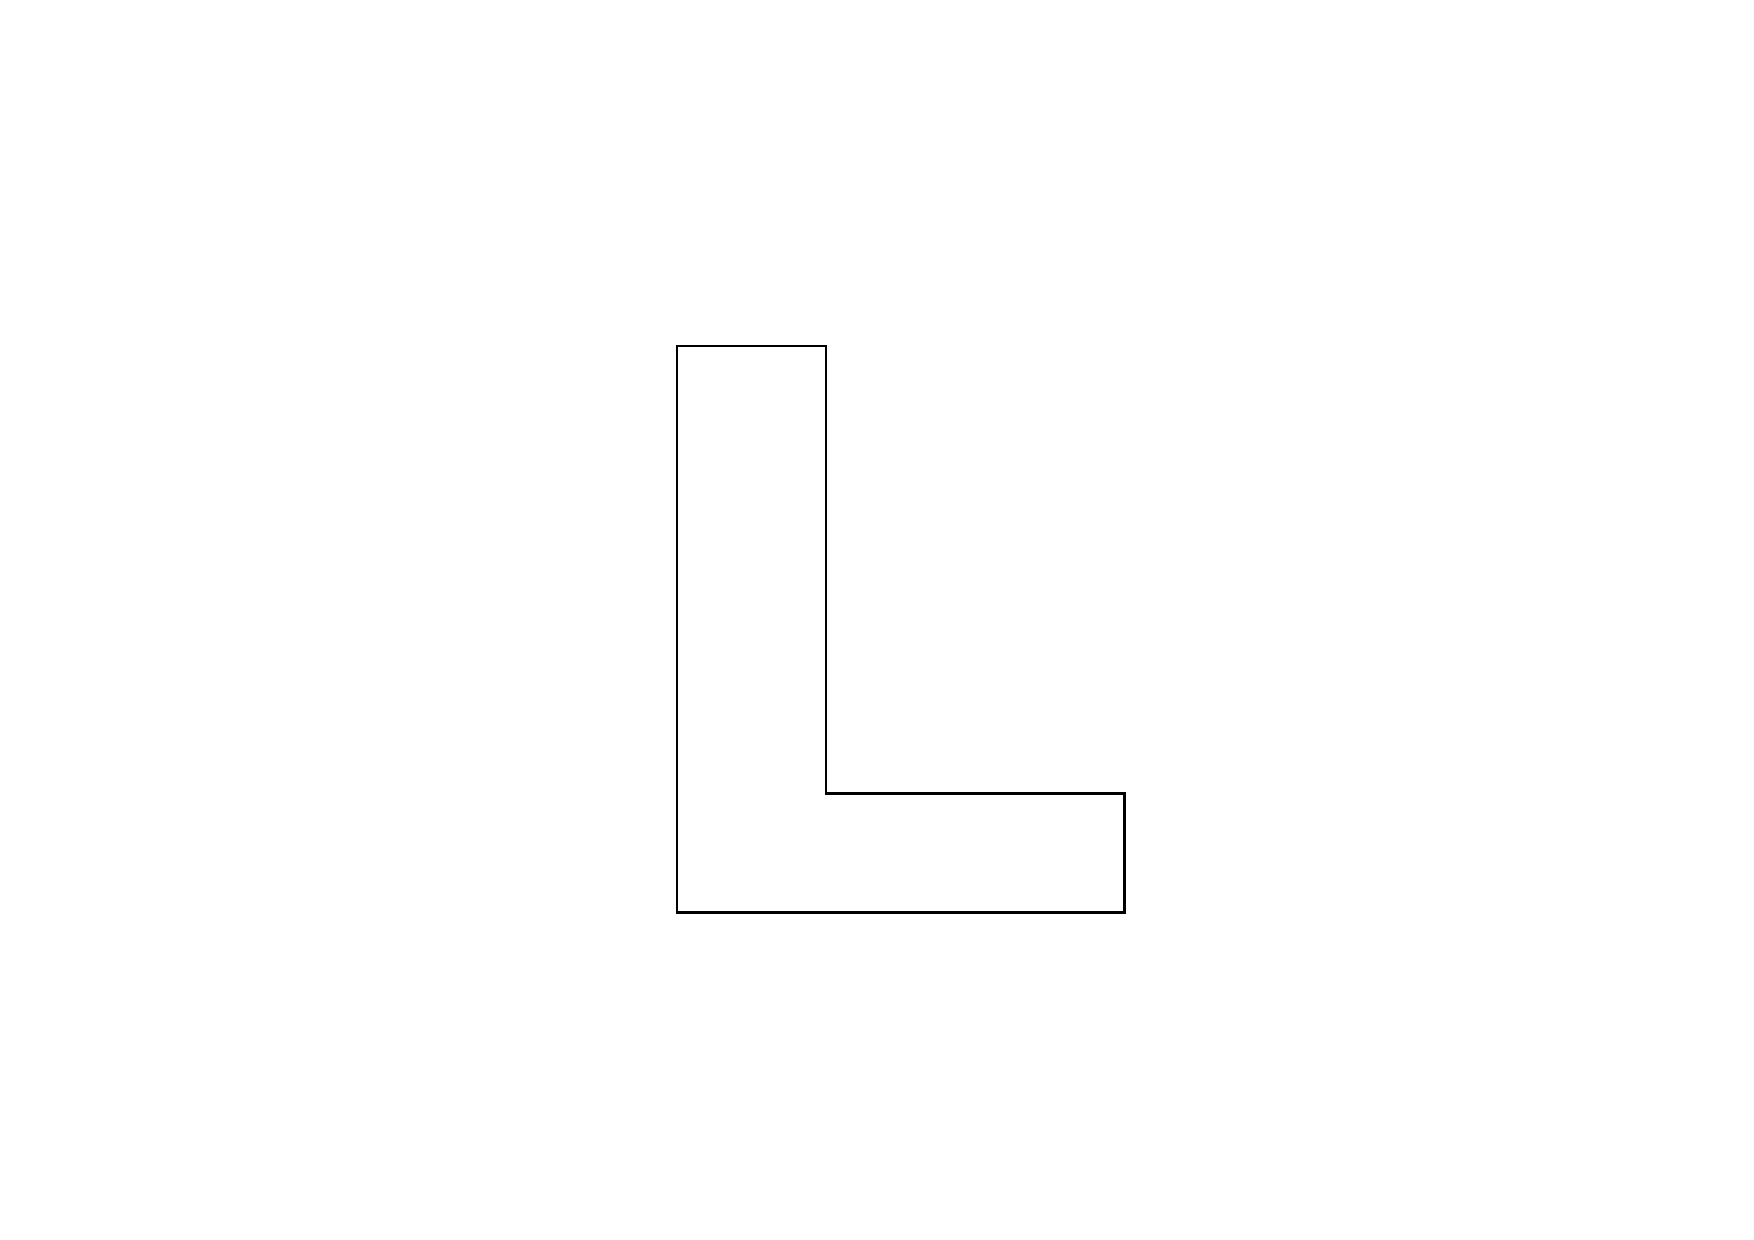
\includegraphics[scale=0.4]{beitezheng.pdf}
\caption{杯零件三维建模基础图}\label{fig:bettezheng}
\end{figure}

\begin{tips}
\item 使用用Line命令过程中,如果由于输入坐标错误或误点鼠标而导线段绘制错误,在没有结束命令前,可以使用U选项撤消上一次绘制的线段。
\item 在使用Line命令过程中,如果还没有绘制完图形就已经结束了命令,可以再次使用直线命令并利用捕捉端点的方式获得需继续绘制点的坐标,然后接着完成图形的绘制。开启端点捕捉的方法有:
\begin{itemize}
\item 绘图过程中在输入坐点时,用键盘输入:end。
\item 绘图过程中按ctrl或shift键+鼠标右击弹出图\ref{fig:duixiangbuzuomen2}所示的【对象捕捉】菜单,并选择【端点】项。
\item 在功能按钮区中将对象捕捉图标由
\includegraphics[scale=0.6]{duixiangbuzuo1.png}状态设置为
\includegraphics[scale=0.6]{duixiangbuzuo.png}状态,并在图标上右击弹出图\ref{fig:duixiangbuzuomen1}所示的【对象捕捉】菜单,并使【端点】项为开启状态。
\end{itemize}
\item 使用坐标和捕捉是实现AutoCAD精确绘图的关键。
\end{tips}
\begin{figure}[htbp]
\centering
\begin{floatrow}
\ffigbox{\caption{“对象捕捉”菜单一}\label{fig:duixiangbuzuomen2}}{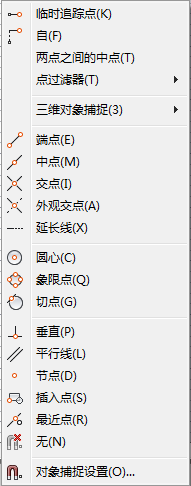
\includegraphics[scale=0.85]{duixiangbuzuomen2.png}}
\ffigbox{\caption{“对象捕捉”菜单二}\label{fig:duixiangbuzuomen1}}{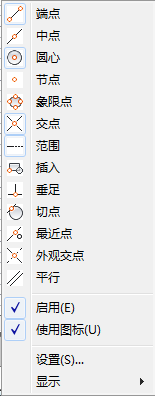
\includegraphics{duixiangbuzuomen1.png}}
\end{floatrow}
\end{figure}

\subsubsection{修改法}
\begin{procedure}
\item 绘制两条相互垂直的直线,作为基础。
\begin{lstlisting}
|命令: LINE|
|指定第一个点:0,15|
|指定下一点或 [放弃(U)]: @0,-15|
|指定下一点或 [放弃(U)]: $@15<0$|
|指定下一点或 [闭合(C)/放弃(U)]: |
\end{lstlisting}
\item 用偏移产生符合尺寸距离的水平线。启动【偏移】命令的方法有:
\begin{itemize}
\item 键盘输入OFFSET或O。
\item 在【修改】菜单中单击【偏移】项。
\item 在【修改】工具栏中单击【偏移】图标
\includegraphics[scale=0.6]{offsettool.png}。
\end{itemize}
\begin{lstlisting}
|命令:OFFSET|
|当前设置: 删除源=否  图层=源  OFFSETGAPTYPE=0|
|指定偏移距离或 [通过(T)/删除(E)/图层(L)] $<$通过$>$:  4|
|选择要偏移的对象,或 [退出(E)/放弃(U)] $<$退出$>$:\longremark{用鼠标选择图\ref{fig:trimmotherd}中的水平线,选中后该水平线将以虚线形式表示,如图\ref{fig:offsetselect}所示。}|
|指定要偏移的那一侧上的点,或[退出(E)/多个(M)/放弃(U)]|
|$<$退出$>$:\longremark{将鼠标移至选中水平线的上方,并单击鼠标左键。}|
|选择要偏移的对象,或 [退出(E)/放弃(U)] $<$退出$>$:|
|命令: OFFSET|
|当前设置: 删除源=否  图层=源  OFFSETGAPTYPE=0|
|指定偏移距离或 [通过(T)/删除(E)/图层(L)] $<4.0000>$:  11|
|选择要偏移的对象,或 [退出(E)/放弃(U)] $<$退出$>$:|
|指定要偏移的那一侧上的点,或 [退出(E)/多个(M)/放弃(U)] |
|$<$退出$>$:|
|选择要偏移的对象,或 [退出(E)/放弃(U)] $<$退出$>$:|
\end{lstlisting}
\showremarks
\item 用偏移产生符合尺寸距离的垂直线。
\begin{lstlisting}
|命令:OFFSET|
|当前设置: 删除源=否  图层=源  OFFSETGAPTYPE=0|
|指定偏移距离或 [通过(T)/删除(E)/图层(L)] $<11.0000>$:  5|
|选择要偏移的对象,或 [退出(E)/放弃(U)] $<$退出$>$:|
|指定要偏移的那一侧上的点,或[退出(E)/多个(M)/放弃(U)]|
|$<$退出$>$:|
|选择要偏移的对象,或 [退出(E)/放弃(U)] $<$退出$>$:|
|命令: OFFSET|
|当前设置: 删除源=否  图层=源  OFFSETGAPTYPE=0|
|指定偏移距离或 [通过(T)/删除(E)/图层(L)] $<5.0000>$:  10|
|选择要偏移的对象,或 [退出(E)/放弃(U)] $<$退出$>$:|
|指定要偏移的那一侧上的点,或 [退出(E)/多个(M)/放弃(U)] |
|$<$退出$>$:|
|选择要偏移的对象,或 [退出(E)/放弃(U)] $<$退出$>$:|
\end{lstlisting}
\begin{figure}[htbp]
\subfloat[]{\label{fig:trimmotherd}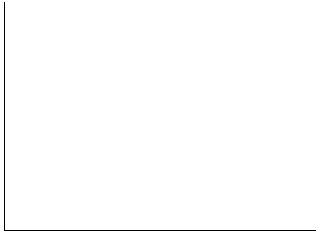
\includegraphics[scale=0.4]{trimmotherd1.png}}\hspace{20pt}
\subfloat[]{\label{fig:offsetselect}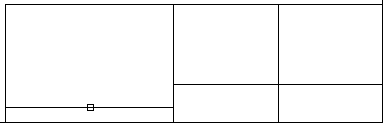
\includegraphics[scale=0.4]{offsetselect.png}}\hspace{20pt}
\subfloat[]{\label{fig:offsetresult}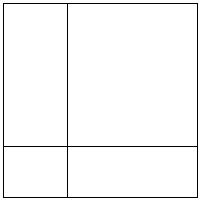
\includegraphics[scale=0.5]{offsetresult.png}}
\caption{偏移过程}
\end{figure}
<<<<<<< HEAD
\item 在完成偏移操作后,其结果如图\ref{fig:offsetresult}所示,现在需要用【修剪】命令修剪掉不需要的线段,以完成图形绘制。【修剪】命令的启动方法有:
\begin{itemize}
\item 解盘输入TRIM或TR。
\item 点击【修改】菜单中的【修剪】项。
\item 点击【修改】工具栏中的【修剪】图标
\includegraphics[scale=0.6]{trimtool.png}。
\end{itemize}
=======
\item 在完成偏移操作后,其结果如图\ref{fig:offsetresult}所示,现在需要用【修剪】命令修剪掉不需要的线段,以完成图形绘制。
>>>>>>> f0e535af97a267194701fe119f482f0290eacbb3
\begin{lstlisting}
|命令: TRIM|
|当前设置:投影=UCS,边=无|
|选择剪切边...|
|选择对象或 $<$全部选择$>$:  指定对角点: 找到 6 个\longremark{以框选方式选择所有的图线用作剪切边,选择方法如图\ref{fig:trimegeselect}所示,选择结果如图\ref{fig:trimselectresult}所示。}|
|选择对象:|
|选择要修剪的对象,或按住 Shift 键选择要延伸的对象,或|
|[栏选(F)/窗交(C)/投影(P)/边(E)/删除(R)/放弃(U)]:  指定对角点:\longremark{以框选方式选择要修剪的对象,选择方法如图\ref{fig:trimedselect}所示,修剪结果如图\ref{fig:trimedresult}所示。}|
|选择要修剪的对象,或按住 Shift 键选择要延伸的对象,或|
|[栏选(F)/窗交(C)/投影(P)/边(E)/删除(R)/放弃(U)]:|
|选择要修剪的对象,或按住 Shift 键选择要延伸的对象,或|
|[栏选(F)/窗交(C)/投影(P)/边(E)/删除(R)/放弃(U)]:|
|选择要修剪的对象,或按住 Shift 键选择要延伸的对象,或|
|[栏选(F)/窗交(C)/投影(P)/边(E)/删除(R)/放弃(U)]:|
\end{lstlisting}
\begin{figure}[htbp]
\subfloat[]{\label{fig:trimegeselect}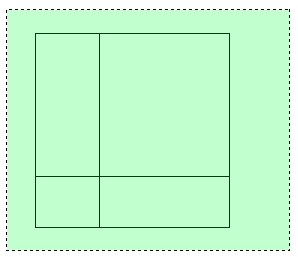
\includegraphics[scale=0.4]{trimegeselect.png}}\hspace{20pt}
\subfloat[]{\label{fig:trimselectresult}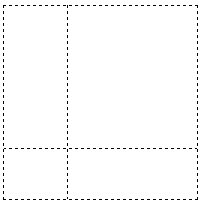
\includegraphics[scale=0.4]{trimselectresult.png}}\hspace{20pt}
\subfloat[]{\label{fig:trimedselect}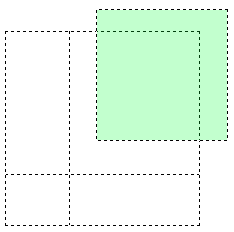
\includegraphics[scale=0.4]{trimedselect.png}}\hspace{20pt}
\subfloat[]{\label{fig:trimedresult}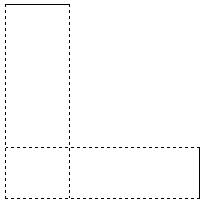
\includegraphics[scale=0.4]{trimedresult.png}}
\caption{修剪过程}
\end{figure}
\showremarks
\end{procedure}
\begin{tips}
\item 【偏移】操作过程中,如果多次偏移的距离相同则可以多次选择对象并执行偏移。
\item 【修剪】操作的关键是修剪边的选择,若要前去某线段之外的其它图线,则应选择该线段作为修剪边;若要剪去某两条线段之间的其它的图线则至少要选择该两条线段,否则不能够实现操作目的。
\item 【修剪】操作中修剪对象的选择具有一定的顺序,般为先剪去外围不需要的图线,再剪去内部的图线,否会出现部分图线不能够剪除,只能够删除的现象。
\end{tips}

\subsection{旋转构建杯零件三维模型}
\begin{procedure}
\item 将图\ref{fig:bettezheng}进行面域。启动【面域】命令的方法有:
\begin{itemize}
\item 解盘输入region或reg。
\item 在【绘图】菜单中单击【面域】项。
\item 在【绘图】工具栏中单击【面域】图标
\includegraphics[scale=0.6]{regiontool.png}。
\end{itemize}
\begin{lstlisting}
|命令:REGION|
|选择对象: 找到 1 个\longremark{已选择一条用以构建封闭区域的对象,被选中的线段以虚线形式表示,其结果如图\ref{fig:regionselecta}所示}|
|选择对象: 找到 1 个,总计 2 个|
|选择对象: 找到 1 个,总计 3 个|
|选择对象: 找到 1 个,总计 4 个|
|选择对象: 找到 1 个,总计 5 个|
|选择对象: 找到 1 个,总计 6 个\longremark{已选择全部6条用以构建封闭区域的对象,构成以虚线表示的封闭框,其结果如图\ref{fig:regionselectb}所示}|
|选择对象:|
\end{lstlisting}
\showremarks
\begin{figure}[htbp]
\centering
\subfloat[]{\label{fig:regionselecta}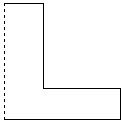
\includegraphics[scale=1.2]{regionselect1.png}}\hspace{30pt}
\subfloat[]{\label{fig:regionselectb}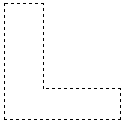
\includegraphics[scale=1.2]{regionselect.png}}
\caption{面域对象选择}
\end{figure}
\item 实体建模中旋转命令完成杯块零件三维模型构建。实体【旋转】命令的启动方法有:
\begin{itemize}
\item 键盘输入revolve或rev。
\item 在【绘图】菜单的【建模】子菜单中单击【旋转】项。
\item 在【建模】工具栏中单击【旋转】图标
\includegraphics[scale=0.6]{solidrevolve.png}。
\end{itemize}
\begin{lstlisting}
|命令: REVOLVE|
|当前线框密度:  ISOLINES=4,闭合轮廓创建模式 = 实体|
|选择要旋转的对象或 [模式(MO)]: 找到 1 个|
|选择要旋转的对象或 [模式(MO)]:|
|指定轴起点或根据以下选项之一定义轴 [对象(O)/X/Y/Z]$<$对象$>$:\longremark{用捕捉方式选择端点用来定义中心线的第一个点,如图\ref{fig:revnodeselecta}所示。}|
|指定轴端点:\longremark{用捕捉方式选择端点用来定义中心线的第二个点,如图\ref{fig:revnodeselectb}所示。}|
|指定旋转角度或 [起点角度(ST)/反转(R)/表达式(EX)] $<360>$:|
\end{lstlisting}
\showremarks
\begin{figure}[htbp]
\centering
<<<<<<< HEAD
\subfloat[]{\label{fig:revnodeselecta}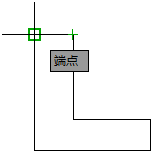
\includegraphics[scale=0.7]{revnodeselect1.png}}\hspace{30pt}
\subfloat[]{\label{fig:revnodeselectb}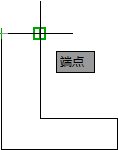
\includegraphics[scale=0.7]{revnodeselect2.png}}
=======
\subfloat[]{\label{fig:revnodeselecta}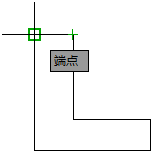
\includegraphics[scale=1.2]{revnodeselect1.png}}\hspace{30pt}
\subfloat[]{\label{fig:revnodeselectb}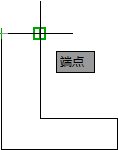
\includegraphics[scale=1.2]{revnodeselect2.png}}
>>>>>>> f0e535af97a267194701fe119f482f0290eacbb3
\caption{旋转中心定义}
\end{figure}
\item 将视图切换为【东南等轴测】,并将【视觉样式】设置为【灰度】即可得到图\ref{fig:beimodel}所示的调压阀杯零件三维模型效果。

切换【东南等轴测】的方法有:
\begin{itemize}
\item 在【视图】菜单【三维视图】子菜单中单击【东南等轴测】项。
\item 在【视图】工具栏中单击【东南等轴测】图标
\includegraphics[scale=0.6]{estool.png}。
\end{itemize}
设置【视觉样式】的方法是:
\begin{itemize}
\item 在【视图】菜单【视觉样式】子菜单中单击【灰度】项。
\end{itemize}
\item 将文件保存为“杯块零件三维图.dwg”。AutoCAD保存文件的方法有:
\begin{itemize}
\item 键盘输入\fbox{Ctrl}+\fbox{S}。
\item 【文件】菜单中【保存】或【另存为】项。
\item 【工具栏】中的【保存】图标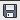
\includegraphics[scale=0.6]{savetool.png}。
\end{itemize}
\end{procedure}
\begin{figure}
\centering
<<<<<<< HEAD
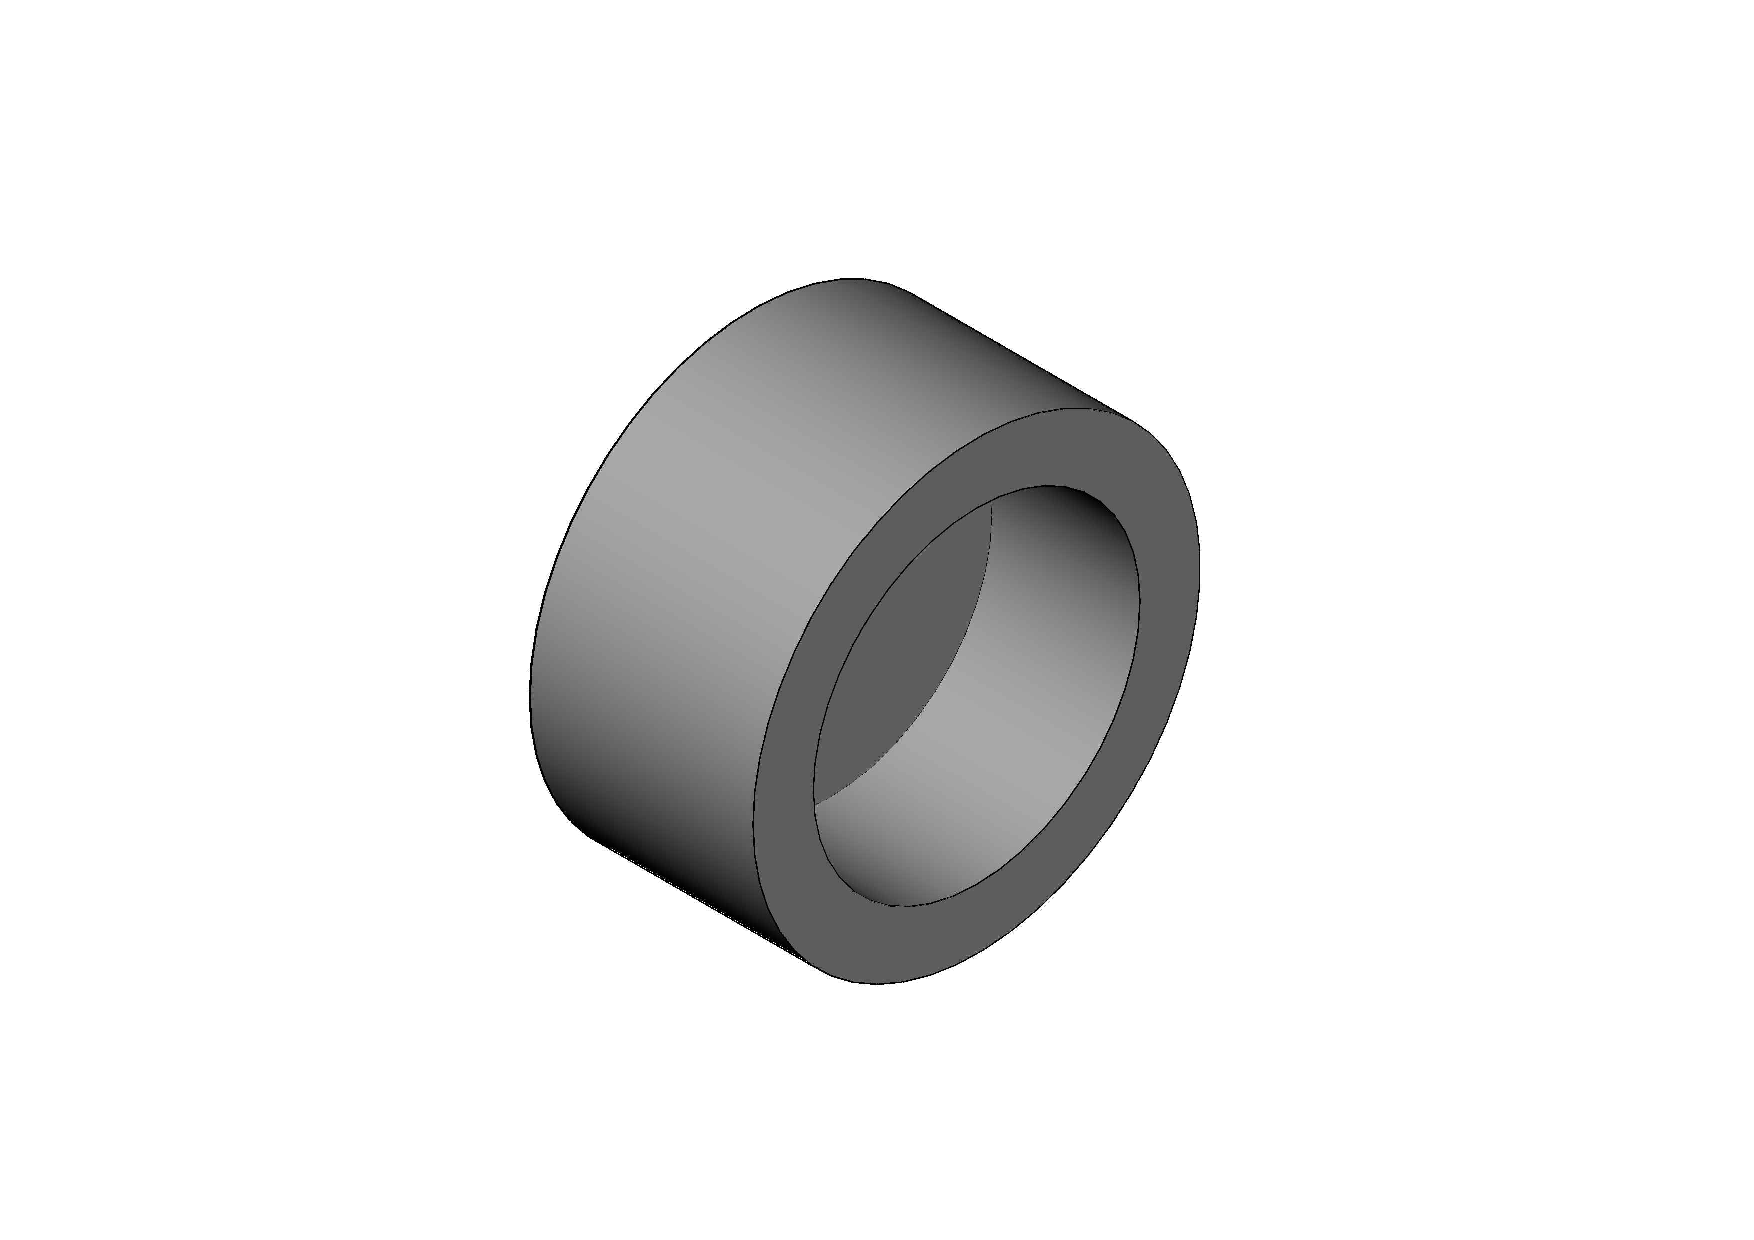
\includegraphics[scale=0.4]{beimodel.pdf}
=======
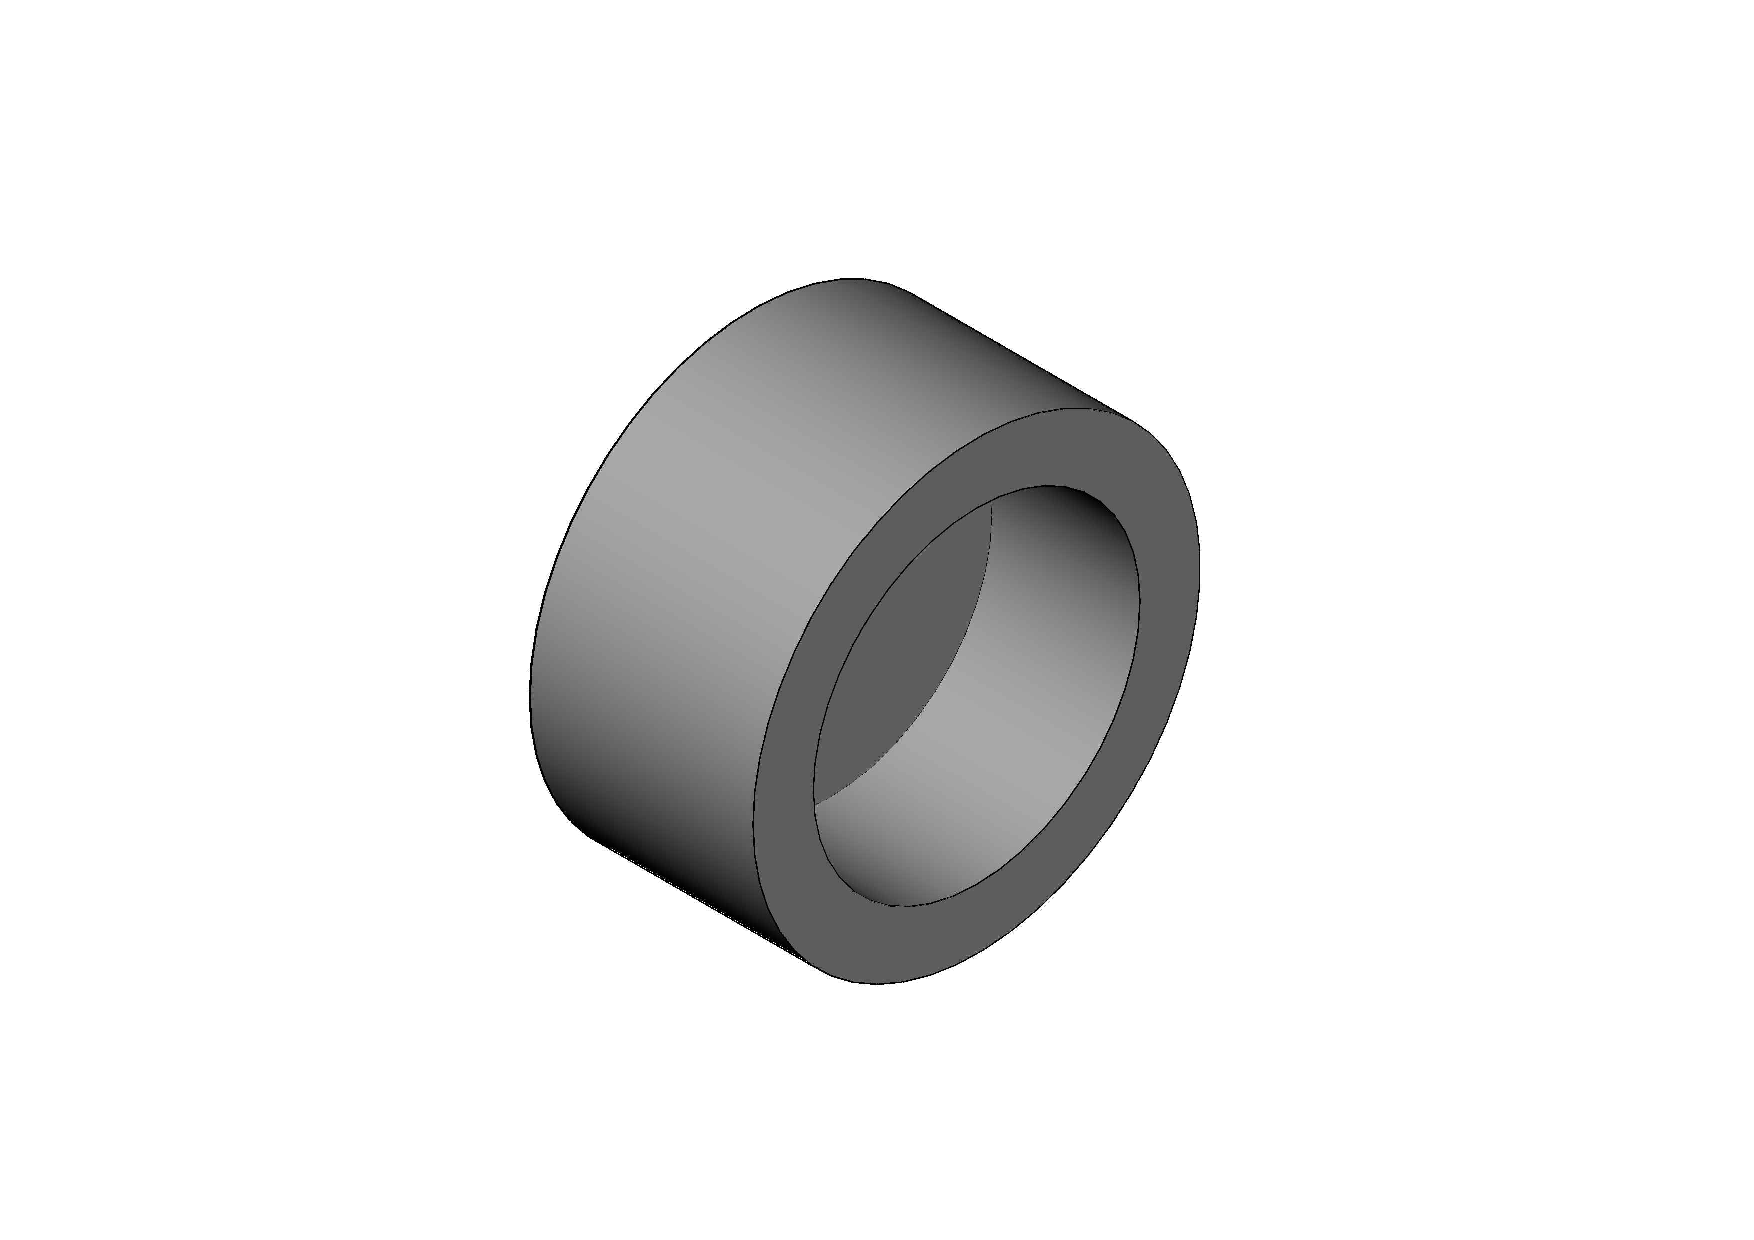
\includegraphics[scale=0.5]{beimodel.pdf}
>>>>>>> f0e535af97a267194701fe119f482f0290eacbb3
\caption{杯零件三维模型}\label{fig:beimodel}
\end{figure}

\begin{tips}
\item 【面域】命令要求选择的线段必须要构成封闭线框,即要求如图\ref{fig:regionselectb}一样,所选择的线段要首尾相接,否则将不能成功面域。
\item 图所示的几种情况都将不能够成功创建面域。
\begin{figure}[htbp]
\centering
\subfloat[]{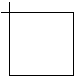
\includegraphics{regerror1.png}}\hspace{20pt}
\subfloat[]{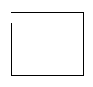
\includegraphics{regerror2.png}}\hspace{20pt}
\subfloat[]{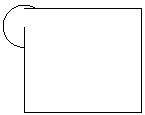
\includegraphics[scale=0.6]{regerror3.png}}\hspace{20pt}
\subfloat[]{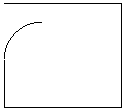
\includegraphics[scale=0.6]{regerror4.png}}
\end{figure}
\item 实体【旋转】命令的角度决定用选定的对象旋转多少度,例如90度将产生四分之一形状的回转体。默认情况下则为360度。
\end{tips}
\endinput